\documentclass[12pt]{extarticle}
\usepackage[english]{babel}
\usepackage{NotesTeX}
\usepackage{subfigure}
\usepackage{tikz}
\usetikzlibrary{arrows}
\usepackage{multirow}
\usepackage{listings}
\usepackage{extarrows}
\usepackage{parskip}
\usepackage{eurosym}
\usepackage{footmisc}

\collaborationImg{
\includegraphics[width=30mm]{../../pictures/UIO.png}}

\author{\Large Håkon Olav Torvik, Vetle Vikenes \& Sigurd Sørlie Rustad}
\title{\Huge Machine Learning: Using regression and neural networks to fit continuous functions and classify data}
\affiliation{\large FYS-STK4155 – Applied Data Analysis and Machine Learning
\\Autumn 2021\\Department of Physics\\University of Oslo\\\\\today}
\begin{document}
\abstract{
	Abstract coming soon.
}
\maketitle
\pagestyle{myplain}
\section{Introduction}
In the modern world, digital data has become one of the most valuable commodities there is. Not because of scarcity, like most other valuables, but rather the exact opposite; the vast abundance of data available makes being able to understand trends and patterns in it extremely valuable for companies looking to expand. However, the data is complex, having many features, and understanding how one affect another is impossible with purely human analysis. Luckily, there exists statistical methods that let us find the deeper connections, make models and even predict outcomes. In this paper we wish to study some of these methods, look at their limitations and strengths.

First we will study a bi-variate continuous function known as the Franke function. We will use both stochastic gradient decent and a feed-forward deep neural network, with back propagation. Then we can also compare results with those obtained in a previous paper, using ordinary least squares and ridge regression. Note that all methods used in this report is briefly covered in the theory section.

Next we will embark on a classification problem, namely wether of not breast tissue is benign or malignant. Here we will also use a feed-forward deep neural network, along with logistic regression.

We will on no way answer all questions linked to the aforementioned methods. Such that anyone can reproduce or continue our studies, we list all the code, results and instructions on running the code in our GitHub repository\footnote{\href{https://github.com/sigurdru/FYS-STK4155/tree/main/project1}{https://github.com/sigurdru/FYS-STK4155/tree/main/project2}}.

\section{Theory}
In the theory-section we aim to give a brief explanation of the main concepts and terminology used in this report. For a more in-depth explanation we recommend reading the appropriate sections in \cite{2019}, which has been of great inspiration and help for us throughout the project.

In general, we have a dataset $\bo x$, where each point $\bo x_i$ takes a value $y_i$, for which we want to make a model $\bbeta$, such that for a new data point $\bo x_k \notin \bo x$ we can make a prediction for the value $y_k$.  The model $\bbeta$ is a vector, where each element is a parameter of our model, such that $\bbeta$ is sometimes called the parameters. For gradient decent, we have to chose what shape the model should be, as was done for linear regression in \cite{project1}, while the neural network makes its own model.

\subsection{Gradient Decent}\label{sec:GD}
In this section we cover gradient decent and different variations of it. More specifically we describe gradient decent (GD), stochastic gradient decent (SGD) and adding momentum to the aforementioned methods. All gradient decent methods start with an initial guess for what the model $\bbeta$ should be, and iteratively updates the guess by training on the dataset, either until it reaches a minimum, or a certain number of iterations have been performed.
\subsubsection{Ordinary Gradient Decent}
Gradient decent methods is often used to minimize the so-called cost/loss-function, which tells us how good our model at predicting the dataset is (more on this in section \ref{sec:cost_func_and_regul}). For now, we use a general cost function $C(\bbeta)$ for a given model $\bbeta$, which can be expressed as the sum over the cost function for each datapoint $\bo x_i$, as such:
\begin{equation}
	C(\boldsymbol{\beta}) = \sum_{i = 1}^{n}c_i(\mathbf{x}_i, \boldsymbol{\beta}),
\end{equation}
where $n$ denotes the number of datapoints. The gradient with respect to the parameters $\bbeta$, which represent the direction of optimal minimization of the cost function,  is then defined as
\begin{align}
	\nabla_{\boldsymbol{\beta}} C(\boldsymbol{\beta}) = \sum_{i = 1}^{n} \nabla_{\boldsymbol{\beta}} c(\mathbf{x}_i, \boldsymbol{\beta}).
	\label{eq:Total_gradient}
\end{align}
The algorithm for GD is then:
\begin{align}
	\mathbf{v}_t             & = \eta \nabla_{\boldsymbol{\beta}} C(\boldsymbol{\beta}_t) \nonumber \\
	\boldsymbol{\beta}_{t+1} & = \boldsymbol{\beta}_t - \mathbf{v}_t,
	\label{eq:GD_algo}
\end{align}
where $\eta$ is what we call the learning rate, representing the step-length to move in the optimal direction.  This algorithms iteratively finds a new $\boldsymbol{\beta}_{t+1}$ which (ideally) decreases the cost function. This is of course not always the case, and depends on the value of $\eta$. For a model with $p$ parameters, the cost-function is the surface of a $p$-dimensional hypersurface, and minimizing this can lead to several problems. For example, if $\eta$  is to big, the cost-function can diverge and never find a minimum of the hypersurface, while if $\eta$ is too small we will need too many iterations to reach a minimum in reasonable time. One method of avoiding the cost-function diverging, is using a dynamic learning schedule, where the learning rate $\eta$ decreases during training. Our model then makes larger steps in the beginning, and then smaller and smaller, such that we should be able to converge to a minimum, and not making too big steps, circling around it.

An additional problem is that the  hypersurface is not a smooth terrain with a single minimum. Our model can potentially move down into a local minimum, which can be close to the level of the global minimum, or far worse than it. When our model converges, we have no way of knowing if we have found the optimal, global minium, or are stuck in one of the many local minima, with no way of getting out.


\subsubsection{Stochastic Gradient Decent}\label{sec:SGD}
With large datasets, a large number of computations is needed when calculating the gradient. It takes a lot of time, and the model is only updated once per iteration, making improvement slow. Stochastic Gradient Decent. SGD, combats this by approximating the total gradient \eqref{eq:Total_gradient}. This is done by performing  gradient decent on a subset of the data, called a minibatch. With $n$ still denoting the total number of datapoints, we will have $N_B=n/M$ minibatches, where $M$ is the size of each minibatch. The minibatches are denoted by $B_k$. Thus our approximated gradient, using a single minibatch $B_k$ is defined as
\begin{align}
	\nabla_{\boldsymbol{\beta}} C^{MB}(\boldsymbol{\beta}) \equiv \sum_{i \in B_k}^M \nabla_{\boldsymbol{\beta}} c(\mathbf{x}_i, \boldsymbol{\beta}).
\end{align}
Then the aim is to use this approximated gradient, for all $N_B$ minibatches, to update the parameters $\boldsymbol{\beta}$, at every step $k$. Doing this for all $N_B$ minibatches, are what we refer to as an epoch. The SGD algorithm then becomes very similar to \eqref{eq:GD_algo}, however with an approximated gradient.
\begin{align}
	\mathbf{v}_t             & = \eta\nabla_{\boldsymbol{\beta}} C^{MB}(\boldsymbol{\beta}_t) \nonumber \\
	\boldsymbol{\beta}_{t+1} & = \boldsymbol{\beta}_t - \mathbf{v}_t
	\label{eq:SGD_algo}
\end{align}
This not only speeds up the algorithms, it also helps prevent getting stuck in local minima because of the stochastic nature. The dataset is shuffled after each epoch, creating new minibatches such that we never use the same one twice.

\subsubsection{Adding Momentum}
These methods can still be optimized further by adding momentum. This is done by adding a term to the parameter $\mathbf{v}_t$ in equations \eqref{eq:GD_algo} and \eqref{eq:SGD_algo}. This so-called mass term, simulates the gradient having momentum, such that every update of $\bbeta$ is a running average.
\begin{align}
	\mathbf{v}_t = \eta \nabla_{\boldsymbol{\beta}_t} C(\boldsymbol{\beta}) \rightarrow \mathbf{v}_t = \gamma \mathbf{v}_{t-1} + \eta \nabla_{\boldsymbol{\beta}} C(\boldsymbol{\beta}_t).
\end{align}
Here $\gamma$ is what we could refer to as the mass, and is a free parameter. One of the benefits is for example that this lets us move faster in regions where the gradient is small.

\subsection{Logistic Regression}\label{sec:logistic_regression}
Gradient decent is used when we have a continuous output, like fitting a function to data. Logistic Regression is used for classification problems, meaning that we want to predict discrete outputs, for instance true or false, given a set of information about a subject. This is the case for binary classification, where we only have one output. It is also possible to use multi-class classification, where one has several outputs, each representing the probability of the class being given by that output.\sn{kanskje flytt denne setningen til senere?} In our case we want a model that takes in some values $\mathbf{x}_i$ and spits out zero or one. These values should correspond to the actual classification $y_i\in\{0,1\}$ corresponding to true or false respectively. Lets define our model as
\begin{align}
	\sigma(s_i), \ \ \text{where }s_i = \bo x_i^T \bo w + b_0 \equiv \bo X_i^T \bo W
	\label{eq:log_reg_model}
\end{align}
Where $\bo x_i^T$ is our data/input, $\bo w$ and $b_0$ are parameters in the model. As a shorthand we also defined $\bo W = (b_0, \bo w)$ and $\bo X_i = (1, \bo x_i)$. We also have $\sigma$ which is some soft classifier that maps our output between zero and one (i.e. the Sigmoid \eqref{eq:sigmoid}). The reason why we want a soft classifier and not a hard one (like $\sigma = 1$ if $s\geq0$ and $0$ otherwise.), is because then we can interpret the output as a probability. Here we also need a cost function to minimize. It is common to choose the cross entropy, which we derive in \ref{sec:cost_func_and_regul}. However we will just use it without derivation for now. The cross entropy for this model is given as
\begin{align}
	C(\bo W) = \sum_{i = 1}^{n} -y_i \log\sigma(\bo X_i^T \bo W) - (1 - y_i)\log\left[1 - \sigma(\bo X^T_i \bo W)\right],
	\label{eq:cross_entropy2}
\end{align}
where $n$ are the number of samples we want to classify. Now with a cost function and model in hand we are ready to minimize the cost function in order to find the optimal parameters for the model. We have a convex cost function, therefore a minimization leads to
\begin{align}
	\nabla_{\bo W} C(\bo W) = \sum_{i = 1}^n \left[\sigma(\bo X_i^T \bo W - y_i)\right]\bo X_i = \bo 0.
\end{align}
Thus the only thing left to do is perform an algorithm similar to \ref{eq:SGD_algo}, where we in this case are updating $\bo W_t$.\sn{RIKTIG?}

\subsection{Feed-Forward Deep Neural Networks}\label{sec:NeuralNetwork}
Neural networks are neural-inspired nonlinear models, which are taught by a way of supervised learning. We will in this section explain what we mean by non-linearity, the basic architecture of a neural network and how the network learns.
\subsubsection{Architecture of Neural Networks}
The structure we are going to use in this report is similar to that in figure \ref{fig:neural_network}. The gray circles are what we refer to as nodes. For now we just need to know that they hold some numerical value. One initializes the network by giving the nodes in the input layer numerical values. These values would correspond to some actual physical property, for example brightness of pixels in a picture. Then, each node in the input layer is connected to each node in the hidden layer $h_1$. In figure \ref{fig:neural_network} we have three such hidden layers, where each node in one layer is connected to every node in the next layer. Now the nodes are connected through what we will refer to as weights, biases and activation functions (more on that later). The connections are what assigns the numerical value of the nodes in the next layer. Lastly we have the output layer, which outputs values dependent on the problem. If we have a classification situation, where we for example wanted to classify the type of animal in different pictures, then one node could correspond to  a lion, next to a zebra and so fourth. By this we would know what animal the network \textit{thinks} is in the picture by looking at what neuron has the highest numerical value.

\begin{figure}[h]
	\minipage{0.70\textwidth}
	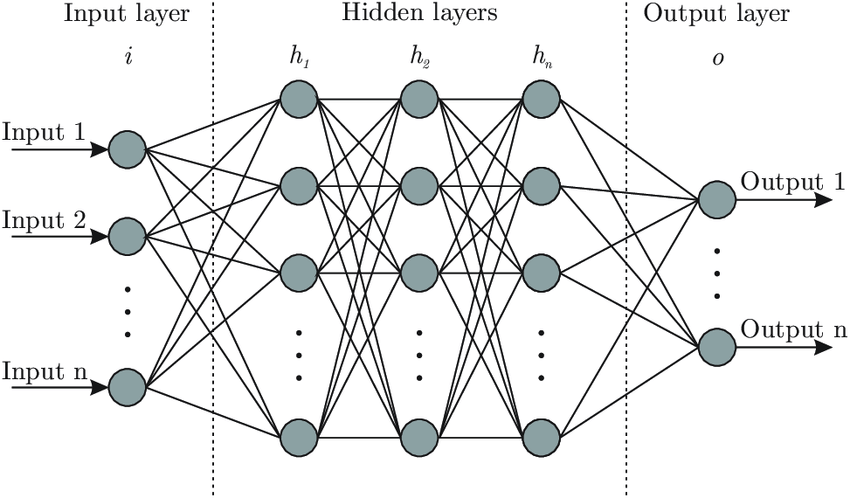
\includegraphics[width=\linewidth]{pictures/neural_network.png}
	(source: \texttt{https://www.researchgate.net/figure/Artificial-neur
		al-network-architecture-ANN-i-h-1-h-2-h-n-o\_fig1\_321259051})
	\endminipage\hfill
	\minipage{0.29\textwidth}
	\caption{Basic outline of a neural network. It displays the different layers (input, hidden and output), nodes (gray circles) and the connection between the nodes (black lines).}\label{fig:neural_network}
	\endminipage
\end{figure}

We mentioned that the different nodes are connected through weights, biases and activation functions. Looking at figure \ref{fig:neural_network}, a neuron $j$ in layer $h_1$ is connected to $n$ input neurons, denoted by black lines. Each input neuron has a numerical value defined by the problem. The value neuron $j$ in $h_1$ then gets is defined as
\begin{align}
	\sigma (x_1w_1 + x_2w_2 + \dots + x_3w_n + b),
\end{align}
where $x_i$ are the values of neuron $i$ in the input layer, $w_i$ are the weights between neurons $i$ and $j$, $b$ is what we refer to as the bias and $\sigma$ is the activation functions (more on them in the next section). Every neuron is connected like this, with different weights and biases. In this project the activation function is the same for each neuron. Note that when we train the data, what we are really doing, is adjusting these parameters to give a desired result. We cover how this is done in the back propagation algorithm section.

\subsubsection{Activation Functions}
The activation functions are where the non-linearity term comes in, because they are non-linear. Now there are many such functions, in our project we have implemented the ones\sn{FLERE?} displayed in figure \ref{fig:activation_functions}. The exact functions are as follows
\begin{align}
	\text{Sigmoid: }\sigma(x)    & = \frac{1}{1 + e^{-x}}\label{eq:sigmoid}           \\
	\text{RELU: }\sigma(x)       & = \max(0,x) \label{eq:RELU}                        \\
	\text{Leaky RELU: }\sigma(x) & = \begin{cases}
		\alpha x, & \text{if } x\leq 0 \\
		x,        & \text{otherwise}
	\end{cases} \label{eq:leaky_RELU}
\end{align}
Where $\alpha$ is some parameter which we have set to $\alpha = 0.01$ in figure \ref{fig:activation_functions}.

\begin{figure}[h]
	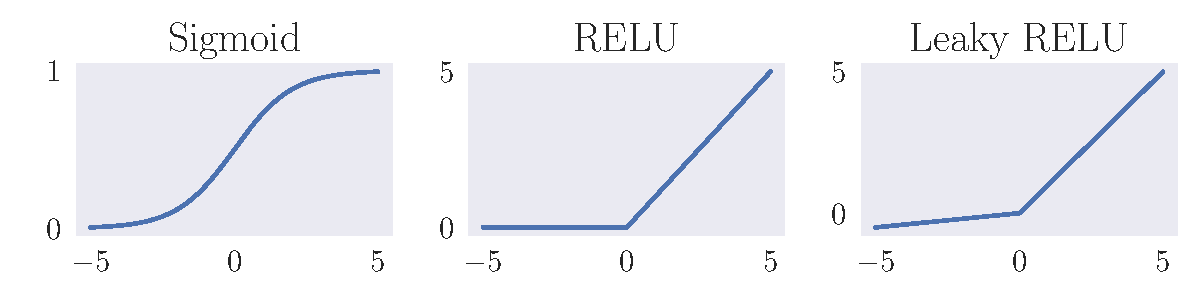
\includegraphics[width=\linewidth]{pictures/activation_functions.pdf}
	\caption{Some activation functions, namely Sigmoid, RELU and Leaky RELU.}\label{fig:activation_functions}
\end{figure}

\subsubsection{Cost Function and Regularization}\label{sec:cost_func_and_regul}
Before one can start training the data, we must have a cost function. This will tell us how well or poorly our network is performing, and is what we want to minimize when we train the network. For continuous data it is common to use mean square error (MSE) as the cost function. Which is just the difference between desired output ($\hat{\mathbf{x}}$) and actual output ($\mathbf{x}$), squared, divided by the number of datapoints $n$ (see equation \eqref{eq:MSE})
\begin{align}
	C(\mathbf{x}) = \frac{1}{n}\sum_{i=1}^{n}(\hat{\mathbf{x}}_i - \mathbf{x}_i)^2.
	\label{eq:MSE}
\end{align}
One can also implement regularization, which helps prevent overfitting in the network. Common ones are $L_1$ and $L_2$ which is done by adding a regularization term to the end of the cost function (see equations \eqref{eq:L1} and \eqref{eq:L2}).
\begin{align}
	L_1: \ \ C(\mathbf{x}) & = \frac{1}{n}\sum_{i=1}^{n}(\hat{\mathbf{x}}_i - \mathbf{x}_i)^2 + \lambda\sum_j \abs{\mathbf{w}_j} \label{eq:L1} \\
	L_2: \ \ C(\mathbf{x}) & = \frac{1}{n}\sum_{i=1}^{n}(\hat{\mathbf{x}}_i - \mathbf{x}_i)^2 + \lambda\sum_j \mathbf{w}^2_j \label{eq:L2}
\end{align}
\sn{RIKTIG?}Here $\lambda$ is some regularization parameter and $\mathbf{w}$ are weights.

We mentioned when talking about logistic regression (section \ref{sec:logistic_regression}), that for classification scenarios one will often use cross-entropy as the cost function. Continuing with the model defined by \eqref{eq:log_reg_model}, we want to find an appropriate cost function. We define the probability of an outcome $y_i$ given parameters $\bo X_i$ and $\bo W$ as
\begin{align}
	P(y_i = 1|\bo X_i, \bo W) & = \frac{1}{1 + \exp(-\bo X_i^T \bo W)}, \\
	P(y_i = 0|\bo X_i, \bo W) & = 1 - P(y_i = 1|\bo X_i, \bo W)
\end{align}
We can then map these probabilities to our soft classifier $\sigma(s_i)$
\begin{align}
	P(y_i = 1) = \sigma(s_i) = \sigma(\bo X_i^T \bo W).
\end{align}
Now we can define the cost function using Maximum Likelihood Estimation (MLE), which states that we should choose parameters that maximize the probability of our given data. Consider the dataset $\mathcal{D}\{(y_i, \bo x_i)\}$, where we remind that $\bo x_i$ are the input parameters. Then the probability of our dataset given $\bo W$ is
\begin{align}
	P(\mathcal{D}|\bo W) = \prod_{i=1}^{n} \left[\sigma(\bo X_i^T\bo W)\right]^{y_i} \left[1 - \sigma(\bo X_i^T\bo W)\right]^{(1 - y_i)}.
\end{align}
Again we remind that $n$ are the number datapoints we want to classify. This expression is difficult to work with, thus we take the logarithm.
\begin{align}
	l(\bo W) = \log(P(\mathcal{D}|\bo W)) = \sum_{i = 1}^n y_i\log(\sigma(\bo X_i^T \bo W)) + (1-y_i)\log(1 - \sigma(\bo X_i^T \bo W))
\end{align}
MLE entails finding the $\bo W$ that maximizes $l(\bo W)$, or more commonly, minimizes $-l(\bo W)$. Thus our cost function becomes
\begin{align}
	C(\bo W) = -l(\bo W) = \sum_{i = 1}^{n} -y_i \log\sigma(\bo X_i^T \bo W) - (1 - y_i)\log\left[1 - \sigma(\bo X^T_i \bo W)\right],
	\label{eq:cross_entropy}
\end{align}
Which is exactly what we wrote down in equation \eqref{eq:cross_entropy2}.
\subsubsection{The Backpropagation Algorithm}
With a desired cost function we are ready to train the neural network. This is done by the backpropagation algorithm. The method entails finding the derivative of the cost function, with respect to all parameters. When we have a neural network, we have thousands of parameters which can be tuned (weights and biases), meaning that we have to approximate the derivative somehow. The backpropagation algorithm does just that, by exploiting the layered structure displayed in figure \ref{fig:neural_network}.

Before we can embark on deriving the algorithm we will introduce some notation. We assume $L$ total layers while $l = 1, \dots , L$ indexes which one. Next we need to index the weights, nodes and biases. Let $w_{jk}^l$ be the weight connecting $k$-th neuron in layer $l-1$ and $j$-th neuron in layer $l$. The index order in $j$ and $k$ are such that we can do matrix multiplication with index notation later down the road. We also let $b_j^l$ be the $j$-th neuron bias in layer $l$. Thus the activation of the $j$-th neuron in layer $l$ ($a^l_j$) becomes
\begin{align}
	a_j^l = \sigma\left(\sum_{k} w_{jk}^l a_k^{l-1} + b_j^l\right) = \sigma(z_j^l), \ \ z_j^l \equiv \sum_{k} w_{jk}^l a_k^{l-1} + b_j^l.
	\label{eq:activation_of_node_ajl}
\end{align}
Here $\sigma$ is an activation function.

Now the cost function will depend directly on the activation of the output layer ($a^L_j$). However the activation of the output layer depends on the previous layers, meaning that the cost function depends indirectly on all the previous layers. Lets define define the error $\Delta_j^L$ of the $j$-th neuron in layer $L$, as the change in cost function with respect to $z^L_j$.
\begin{align}
	\Delta_j^L \equiv \del{C}{z_j^L}
	\label{eq:backprop0}
\end{align}
We can similarly define the error of neuron $j$ in layer $l$ ($\Delta_j^l$), as the change in the cost function with respect to $z_j^l$,
\begin{align}
	\Delta_j^l \equiv \del{C}{z_j^l} = \del{C}{a_j^l}\del{a_j^l}{z^l_j} = \del{C}{a_j^l}\der{\sigma(z^l_j)}{z^l_j}.
	\label{eq:backprop1}
\end{align}
In the next few lines we are going to derive several equations needed for the algorithm, it will be apparent why after we have found them. Notice that \eqref{eq:backprop1} also can be written as
\begin{align}
	\Delta_j^l = \del{C}{z_j^l} = \del{C}{b_j^l}\del{b_j^l}{z^l_j} = \del{C}{b_j^l}.
	\label{eq:backprop2}
\end{align}
Because $\partial b_j^l/\partial z^l_j = 1$ from \eqref{eq:activation_of_node_ajl}. Again using the chain rule we can rewrite \eqref{eq:backprop1}
\begin{align}
	\Delta_j^l & = \del{C}{z_j^l} = \sum_{k} \del{E}{z_k^{l+1}}\del{z_k^{l+1}}{z^l_j} = \sum_{k} \Delta_k^{l+1}\del{z_k^{l+1}}{z^l_j} \nonumber \\
	           & = \left(\sum_{k} \Delta_k^{l+1} w_{kj}^{l+1}\right)\der{\sigma(z^l_j)}{z^l_j}.
	\label{eq:backprop3}
\end{align}
To find the last equation, we differentiate the cost function with respect to the weight $w^l_{jk}$
\begin{align}
	\del{C}{w_{jk}^l} = \del{C}{z_j^l}\del{z_j^l}{w_{jk}^j} = \Delta l a_k^{l-1}.
	\label{eq:backprop4}
\end{align}
Now why have we done all this work, well because the equations \eqref{eq:backprop1}, \eqref{eq:backprop2}, \eqref{eq:backprop3} and \eqref{eq:backprop4} define what we call the backpropagation algorithm. Then, what exactly is the algorithm? In entails six steps:
\begin{description}
	\item[1 Activation:] First activate the neurons in the activation layer ($a^1_j$) with desired data.
	\item[2 Feedforward:] Activate the nodes in following layers, this is done by equation \eqref{eq:activation_of_node_ajl}.
	\item[3 Error at layer $L$:] Calculate the error at the last layer using \eqref{eq:backprop1}.
	\item[4 Backpropagate error:] With \eqref{eq:backprop3} we can the calculate the error, iterating backwards in the network.
	\item[5 Calculate gradient:] Find the gradient by using equations \eqref{eq:backprop2} and \eqref{eq:backprop4}.
	\item[6 Update parameters:] Update the parameters similarly to \eqref{eq:SGD_algo}, however $\boldsymbol{\beta}_t$ are our weights and biases in this case.\sn{RIKTIG?}
\end{description}

\subsubsection{Initialization of weights}
We mentioned earlier than then the network is created, it has weights and biases between the layers. These needs to be initialized in some way. The biases are simple to initialize, as they are a single number for every node. These are initialized as a small, non-zero value $b_0$, which we choose as $b_0=0.01$.

Before 2006, most neural networks were performing quite badly on most tasks, as they did not learn during training. One of the (several) reasons were due to bad initialization of weights. A common way of doing this was using the standard normal distribution $W_{i,j} \sim  \mathcal{N}(0, 1)$. The problem with this is that it does not consider the size of the layers. In 2010, it was shown that when using sigmoid as the activation function, Xavier-initialization give better results \cite{xavier}. This is given as $W_{i, j}\sim\mathcal{U} \left(-\frac{1}{\sqrt{n}}, \frac{1}{\sqrt{n}} \right)$, where $\mathcal{U}$ is the uniform distribution, and $n$ is the number of nodes in the preceding layer.

In 2015, He-initialization was shown to work well with ReLU and Leaky ReLU \cite{He}. Here, the weights are initialized using the normal distribution, but with a variance given by $v = 2/(1 + \alpha^2)n$, where again $n$ is the number of nodes in the preceding layer, and $\alpha$ is the parameter of the Leaky ReLU-function. For ReLU, this is 0. We use these initializations for our weights given the activation-function, but will not study the particular effects of this in depth.


\section{Methods}
As we mentioned in the introduction, we wish to study different ways of fitting two types of datasets. The first which we can classify as \textit{continuous} is the Franke Function \eqref{eq:FF},
\begin{align}
	\begin{split}\label{eq:FF}
		f(x,y) = &\frac{3}{4}\exp(-\frac{(9x -2)^2}{4} - \frac{(9y-2)^2}{4}) + \frac{3}{4}\exp(-\frac{(9x + 1)^2}{49} - \frac{(9y + 1)}{10})
		\\
		+ &\frac{1}{2}\exp(-\frac{(9x-7)^2}{4} - \frac{(9y -3)}{4}) - \frac{1}{5}\exp(-(9x-4)^2 - (9y-7)^2).
	\end{split}
\end{align}
We will use both stochastic gradient decent and feed forward neural network to try and fit the data. Both methods are covered in the theory sections \ref{sec:GD} and \ref{sec:NeuralNetwork} respectively.

Next we will embark on an classification problem. Namely classifying if breast tissue is malignant or benign, by studying the data provided by Wisconsin breast cancer data\footnote{\href{https://www.kaggle.com/uciml/breast-cancer-wisconsin-data}{https://www.kaggle.com/uciml/breast-cancer-wisconsin-data}}. We will again use a feed forward neural network, and logistic regression. The latter is covered in the theory section \ref{sec:logistic_regression}.

\subsection{Franke Function}
In \cite{project1}, we already studied the Franke function using linear regression, specifically OLS and OLS with an L2 and L1 parameter $\lambda$, so-called Ridge and Lasso regression. The results from these methods will form the basis for comparing our results using SGD and neural networks. The rapport, along with the code can be found at our GitHub\footnote{https://github.com/sigurdru/FYS-STK4155/tree/main/project1}. In order to have comparable results, we will use the same parameters for the data. Only the methods will be different. In that project we initialized the data with $N=30\times30$ randomly (uniformly) distributed datapoints in $x$- and $y$-direction. To simulate it being real data, we also added normally distributed noise with mean zero and standard deviation $0.2$: $\epsilon \sim \mathcal{N}(0,0.2)$. We also scale the data in the same way as before, subtracting the mean and dividing by the standard deviation.

\subsubsection{Stochastic Gradient Descent}
As in \cite{project1}, we have to choose a model to fit the data to, when using SGD. The simplest is a bi-variate polynomial of degree $P$, such that our model will have $p$ features. This is the designmatrix $X$ used in the previous project. Having obtained good results for OLS using $P = 7$, we use the same polynomial degree for SGD. Writing our own code for implementing SGD, and perform an analysis of the MSE (equation \eqref{eq:MSE}) for different learning rates $\eta$ and $L_2$-regularization-parameter $\lambda$.


The specific parameters we will test for are\sn{HVILKE PARAMETERE VI TESTER FOR HER}

\subsubsection{Feed Forward Neural Network}
When using the neural network to fit the Franke function, we use a lot of the same methods as for SGD. A key difference is that instead of iteratively updating a model $\bbeta$, we now train a network of several layers, each with many nodes. One of the results of this is that we do not have to choose the shape the model will take. Instead of giving our network the design matrix $X$ for a cartain polynomial degree $P$, we can pass it only the collection of points $[(x_i, y_i)]$, and let the network figure out the rest. By giving it the entire design matrix, we would pass more data, making it potentially learn better or quicker. If our data were of a physical nature, it would be benefitial, to constrain the predictions to within the laws of nature, which obviously have to be observed. The Franke function is however a pure mathematical object, so no constraints have to be made. We therefore only pass it the $x_i$ and $y_i$  values.
Next we want to perform the same analysis, using a feed forward neural network and back propagation. We perform tests with different number of hidden layers and nodes. Also...

\subsection{Wisconsin Breast Cancer Data}
\subsubsection{Feed Forward Neural Network}
\subsubsection{Logistic Regression}

\section{Results}

%Section ideas:
%\subsection{Franke Function}
%\subsubsection{Stochastic Gradient Descent}
%\subsubsection{Feed Forward Neural Network}
%
%\subsection{Wisconsin Breast Cancer Data}
%\subsubsection{Feed Forward Neural Network}
%\subsubsection{Logistic Regression}

\section{Discussion}

\section{Conclusion}
\appendix
\section{Appendix}
\bibliographystyle{plain}
\bibliography{refs}
\end{document}

